\documentclass[a4paper, 10pt]{article}
\usepackage[left=2.5cm,top=3cm,right=2.5cm,bottom=2.5cm]{geometry}


\usepackage[utf8]{inputenc}
\usepackage{ragged2e}  
\usepackage{cancel}
\usepackage{mathrsfs}
\usepackage{amsmath}
\usepackage{graphicx}
\usepackage{array}
\usepackage{hyperref}
\usepackage[spanish]{babel}
\usepackage{multicol}
\usepackage{amssymb}
\usepackage[usenames,dvipsnames,svgnames,table]{xcolor}
\usepackage{dsfont}
\usepackage{parskip}

\begin{document}
	
	La mínima escala del Vernier es $\dfrac{0.01 cm}{2}=0.005 cm$.\\\\
	La mínima escala de la cinta métrica es $\dfrac{0.1 cm}{2}=0.05 cm$
	
	PARTE A
	
	Se obtuvo que la distancia imagen $s_i$ del Sol con la lente era $s_i=(10.41\pm0.005)cm$. Entonces
	$$\dfrac{1}{s_o}+\dfrac{1}{s_i}=\dfrac{1}{f}\Longrightarrow\dfrac{1}{\infty}+\dfrac{1}{(10.41\pm0.005) cm}=\dfrac{1}{f}\Longrightarrow f=(10.41\pm0.005) cm$$
	$$\therefore f=(10.41\pm0.005) cm$$
	
	PARTE B
	
	Los resultados de realizar las mediciones correspondientes a las distancias objeto e imagen fueron las siguientes

	\begin{table}[ht]
		\centering
		\caption{Distancia objeto $d_o$ y distancia imagen $d_i$ medidas en cada experimento conforme se modificaba la distancia desde la fuente de luz.}	
		\begin{tabular}{|c|c|c|}
			\hline
			Distancia desde la fuente de luz (cm) & $ (d_o \pm 0.05) cm$ & $(d_i \pm 0.05)cm$ \\
			\hline
			100 & 88.9 & 11.1 \\
			\hline
			100 & 10.2 & 89.8 \\
			\hline
			90 & 78.9 & 11.1 \\
			\hline
			90 & 10.4 & 79.6 \\
			\hline
			80 & 68.6 & 11.4 \\
			\hline
			80 & 10.5 & 69.5 \\
			\hline
			70 & 58.5 & 11.5 \\
			\hline
			70 & 10.8 & 59.2 \\
			\hline
			60 & 47.85 & 12.15 \\
			\hline
			60 & 11.3 & 48.7 \\
			\hline
			50 & 36.65 & 13.35 \\
			\hline
			50 & 12.2 & 37.8 \\
			\hline
		\end{tabular}
	\label{tab:exp2}
	\end{table}

	Luego, se calcularon los recíprocos de la distancia objeto $d_o$ y la distancia imagen $d_i$ (el cálculo de la incertidumbre se encuentra en la sección ...).
	\begin{table}[ht]
	\centering
	\caption{Recíprocos de las mediciones obtenidas.}		
		\begin{tabular}{|c|c|c|c|c|}
			\hline & & & &\\
			Distancia $(cm)$ & $(d_o \pm 0.05) cm$ & $\dfrac{1}{(d_o \pm 0.05)} cm^{-1}$ & $(d_i \pm 0.05) cm$ & $\dfrac{1}{(d_i \pm 0.05)} cm^{-1}$ \\ & & & &\\
			\hline
			$100$ & 88.9 & $0.0112\pm6.3265\times10^{-6}$ & 11.1 & $0.0900\pm4.0581\times10^{-4}$ \\
			\hline
			$100$ & 10.2 & $0.0980\pm4.8058\times10^{-4}$ & 89.8 & $0.0111\pm6.2003\times10^{-6}$ \\
			\hline
			$90$ & 78.9 & $0.0126\pm8.0318\times10^{-6}$ & 11.1 & $0.0900\pm4.0581\times10^{-4}$ \\
			\hline
			$90$ & 10.4 & $0.0961\pm4.6227\times10^{-4}$ & 79.6 & $0.0125\pm7.8912\times10^{-6}$ \\
			\hline
			$80$ & 68.6 & $0.0145\pm1.0624\times10^{-5}$ & 11.4 & $0.0877\pm3.8473\times10^{-4}$ \\
			\hline
			$80$ & 10.5 & $0.0952\pm4.5351\times10^{-4}$ & 69.5 & $0.01438\pm1.0351\times10^{-5}$ \\
			\hline
			$70$ & 58.5 & $0.0170\pm1.4610\times10^{-5}$ & 11.5 & $0.0869\pm3.7807\times10^{-4}$ \\
			\hline
			$70$ & 10.8 & $0.0925\pm4.2866\times10^{-4}$ & 59.2 & $0.0168\pm1.4266\times10^{-5}$ \\
			\hline
			$60$ & 47.85 & $0.0208\pm2.1837\times10^{-5}$ & 12.15 & $0.0823\pm3.3870\times10^{-4}$ \\
			\hline
			$60$ & 11.3 & $0.0884\pm3.9157\times10^{-4}$ & 48.7 & $0.0205\pm2.1082\times10^{-5}$ \\
			\hline
			$50$ & 36.65 & $0.0272\pm3.7223\times10^{-5}$ & 13.35 & $0.0749\pm2.8054\times10^{-4}$ \\
			\hline
			$50$ & 12.2 & $0.0819\pm3.3593\times10^{-4}$ & 37.8 & $0.0264\pm3.4993\times10^{-5}$ \\
			\hline
		\end{tabular}
	\end{table}
	\newpage
	Aplicando el método de mínimos cuadrados, se obtuvo que la ecuación de la recta que mejor se ajusta a las observaciones $\dfrac{1}{d_o}$ y $\dfrac{1}{d_i}$ es
	
	$$\dfrac{1}{d_o}=(-1.0925\pm 0.0068)\left(\dfrac{1}{d_i}\right)+(0.1105\pm 0.0004)cm^{-1}$$
	
	Su correspondiente análisis dimensional se discute en el apéndice, sección [no sé]. 
	
	Gráficamente
	
	\begin{figure}[ht]
		\centering
		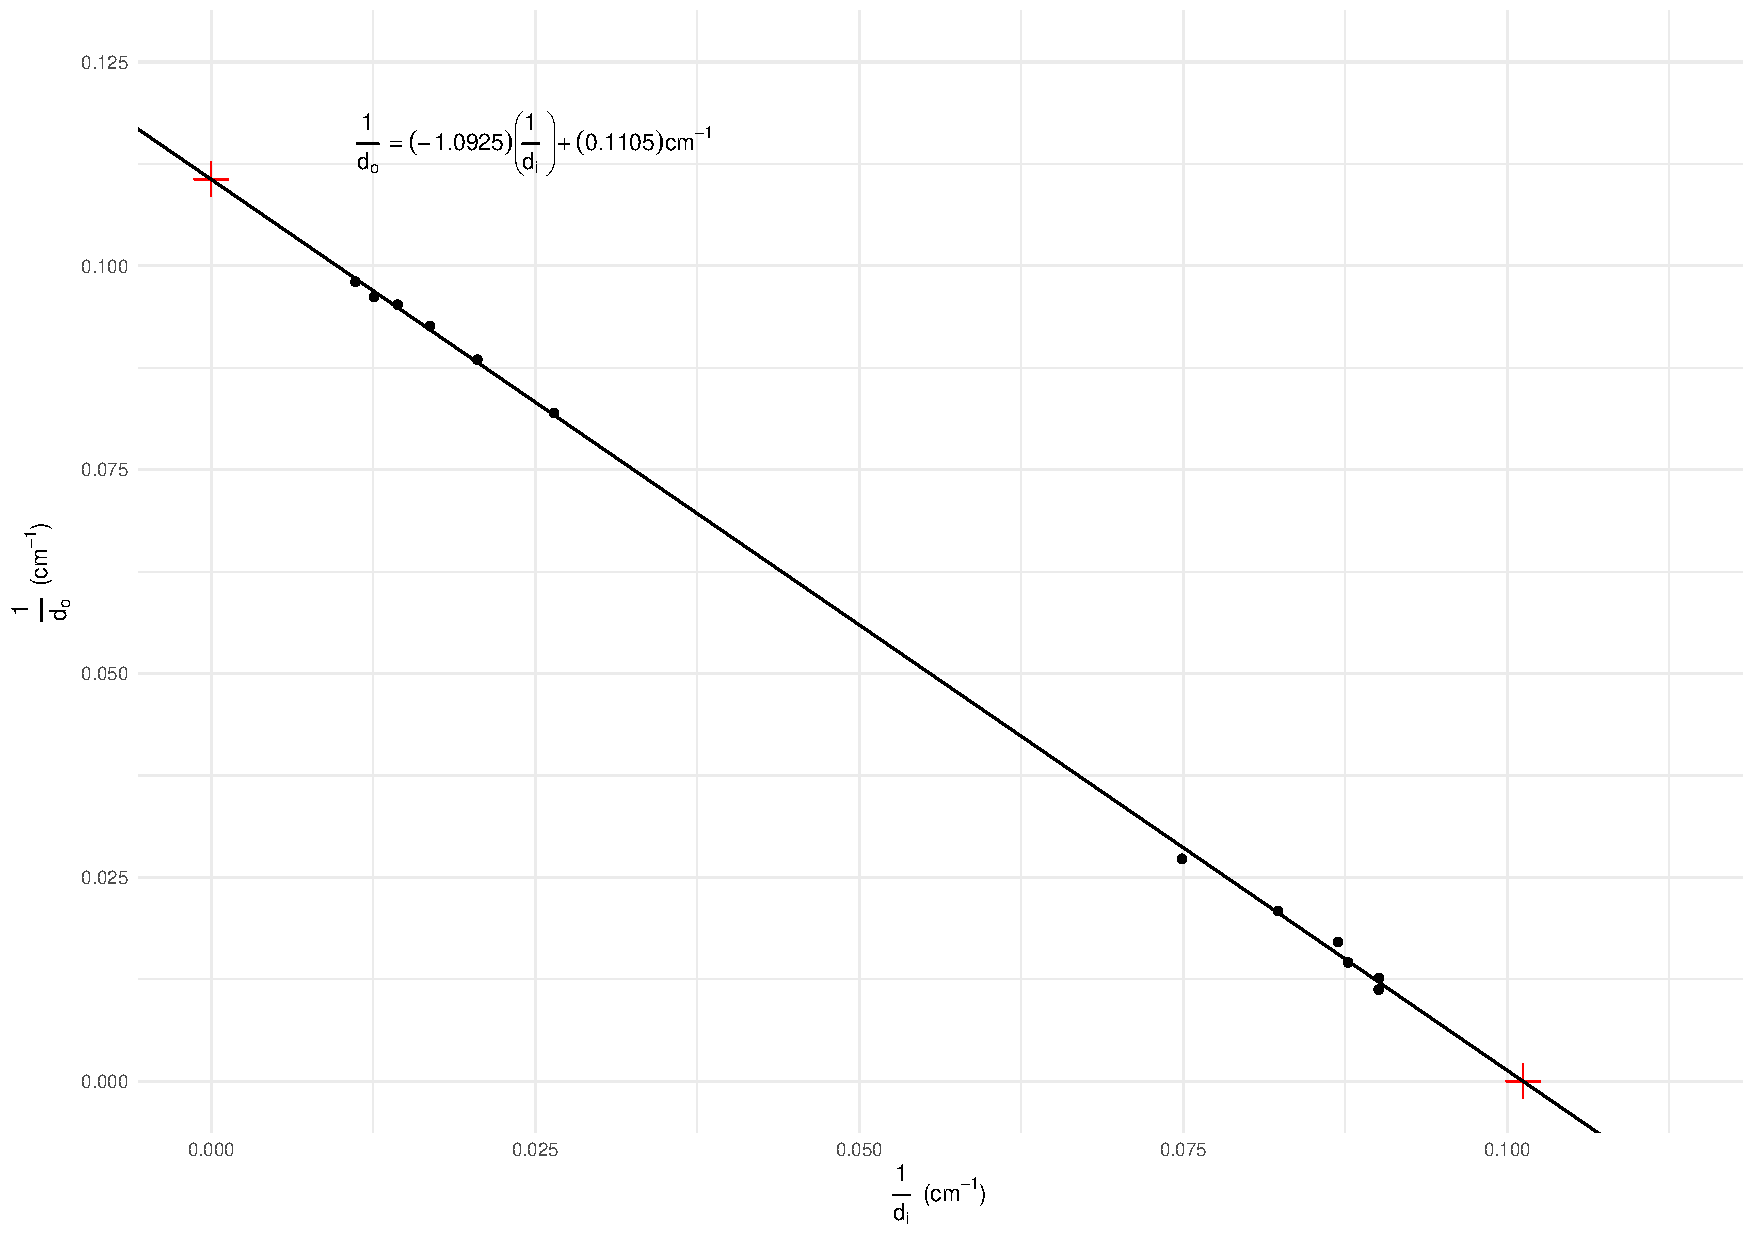
\includegraphics[width= 1\linewidth]{graf1.pdf}
		\caption{$\dfrac{1}{d_o}$ vs \(\dfrac{1}{d_i}\).}
		\label{fig:identidad}
	\end{figure}
	
	Luego, se tiene que
	
	\begin{multicols}{2}
		\begin{itemize}
			\item Intersección con el eje de las ordenadas
			$$\dfrac{1}{d_i}=(0.1012\pm 0.0010) cm^{-1}$$
			
			\item Intersección con el eje de las abscisas
			$$\dfrac{1}{d_o}=(0.1105\pm 0.0004) cm^{-1} $$
		\end{itemize}
	\end{multicols}
	
	Y con estos resultados se obtuvo lo siguiente	
	\newpage
		
	\begin{table}[ht]
		\centering
		\caption{Cálculos de la distancia focal.}
		\begin{tabular}{|c|c|}
		\hline
		Calcular a partir de: & Distancia focal \\
		\hline
		Intersección con eje $x$ & $(9.8814\pm0.0976)cm$\\ 
		\hline
		Intersección con eje $y$ & $(9.0497\pm 0.0818)cm$\\ 
		\hline
		$\%$ de diferencia entre valores anteriores & $|9.8814-9.0497|\times 100\% =83.17\% $\\
		\hline
		Promedio de valores calculados  & $\dfrac{((9.8814+9.0497)\pm (0.0976+0.0818))cm}{2}=$\\
		del eje $x$ y eje $y$ & \\
		& $=(9.4655\pm 0.0897)cm$ \\
		\hline
		Resultado de la parte A & $(10.41\pm0.005) cm$ \\
		\hline
		$\%$ de diferencia entre el valor calculado como & \\
		el promedio de los valores del eje $x$ y eje $y$ & $|9.4655-10.41|\times 100\% =94.44\%$ \\
		y el resultado de la parte A & \\
		\hline
	\end{tabular}
	\end{table}

	PARTE C
	
	Para cada una de las distancias objeto ($d_o$) e imagen ($d_i$) se registraron los siguientes tamaño objeto ($y_o$) y tamaño imagen ($y_i$)  
	
	\begin{table}[ht]
	\centering
	\caption{Tamaño objeto y tamaño imagen correspondientes a cada observación de la distancia objeto $d_o$ y distancia imagen $d_i$.}	
	\begin{tabular}{|c|c|c|c|c|}
			\hline Distancia desde la&&&&\\
			 fuente de luz (cm) & $ (d_o \pm 0.05) cm$ & $(d_i \pm 0.05)cm$ & $ (y_i \pm 0.005) cm$ & $ (y_o \pm 0.005) cm$ \\
			\hline
			100 & 88.9 & 11.1 & $-$0.54 & 4 \\
			\hline
			100 & 10.2 & 89.8 & $-$8.18 & 1 \\
			\hline
			90 & 78.9 & 11.1 & $-$0.83 & 4  \\
			\hline
			90 & 10.4 & 79.6 & $-$7.02 & 1  \\
			\hline
			80 & 68.6 & 11.4 & $-$0.7 & 4  \\
			\hline
			80 & 10.5 & 69.5 & $-$6.02 & 1  \\
			\hline
			70 & 58.5 & 11.5 & $-$0.83 & 4  \\
			\hline
			70 & 10.8 & 59.2 & $-$4.925 & 1  \\
			\hline
			60 & 47.85 & 12.15 & $-$1.03 & 4  \\
			\hline
			60 & 11.3 & 48.7 & $-$3.9 & 1  \\
			\hline
			50 & 36.65 & 13.35 & $-$1.7 & 4 \\
			\hline
			50 & 12.2 & 37.8 & $-$2.845 & 1 \\
			\hline
		\end{tabular}
		\label{tab:parte c}
	\end{table}
	\newpage 
	A partir de estos valores se calcularon los aumentos de la lente (magnificación) y su porcentaje de diferencia
	\begin{table}[ht]
	\centering
	\caption{Cálculo de la magnificación a partir de los datos obtenidos}	
	\begin{tabular}{|c|c|c|}
		\hline &&\\
		$M_1=-\dfrac{(d_i \pm 0.05) cm}{(d_o \pm 0.05)cm}$ & $M_2=\dfrac{(y_i \pm 0.05) cm}{(y_o \pm 0.05)cm}$ & $\left||M_1|-|M_2|\right|\times100\%$ \\ &&\\
		\hline
		$-0.1248\pm0.0006$ & $-0.1350\pm0.0014$ &  $1.01\%$ \\
		\hline
		$-8.8039\pm0.0480$ & $-8.1800\pm0.0459$ &  $62.39\%$ \\
		\hline
		$-0.1406\pm0.0007$ & $-0.2075\pm0.0015$ &  $6.68\%$ \\
		\hline
		$-7.6538\pm0.0416$ & $-7.0200\pm0.0401$ &   $63.38\%$ \\
		\hline
		$-0.1661\pm0.0008$ & $-0.1750\pm0.0014$ &   $0.88\%$ \\
		\hline
		$-6.6190\pm0.0362$ & $-6.0200\pm0.0351$ &   $59.90\%$ \\
		\hline
		$-0.1965\pm0.0010$ & $-0.2075\pm0.0015$ &   $1.09\%$ \\
		\hline
		$-5.4814\pm0.0300$ & $-4.9250\pm0.0296$ &   $55.64\%$ \\
		\hline
		$-0.2539\pm0.0013$ & $-0.2575\pm0.0015$ &  $0.35\%$ \\
		\hline
		$-4.3097\pm 0.0234$ & $-3.9000\pm0.0245$ &  $40.97\%$ \\
		\hline
		$-0.3642\pm0.0018$ & $-0.4250\pm0.0017$ &  $6.07\%$ \\
		\hline
		$-3.0983\pm0.0167$ & $-2.8450\pm0.0192$ &  $25.33\%$ \\
		\hline
	\end{tabular}
	\label{tab:magnificación}
	\end{table}	


	\newpage
	CÁLCULO INCERTIDUMBRE
	
	La incertidumbre para un cociente está dada por
	$$\dfrac{x\pm\delta x}{y\pm\delta y}=\dfrac{x}{y}\pm\left(\dfrac{\delta x}{|y|}+|x|\dfrac{\delta y}{|y|^2}\right)$$
	
	Sin embargo, para este caso el numerador no se trataba de una observación, sino de un número fijo, por lo que $\delta x=0$. Así pues, el cálculo de la incertidumbre para el cociente quedaría
	$$\dfrac{x}{y\pm0.05}=\dfrac{x}{y}\pm|x|\dfrac{0.05}{|y|^2}$$

	INCERTIDUMBRE PARTE B
	
	Para las observaciones referentes a la distancia objeto $d_o$
	\begin{align*}
		\dfrac{1}{88.9\pm 0.05}&=\dfrac{1}{88.9}\pm\dfrac{0.05}{88.9^2}=0.0112\pm6.3265\times10^{-6}\\\\
		\dfrac{1}{10.2\pm 0.05}&=\dfrac{1}{10.2}\pm\dfrac{0.05}{10.2^2}=0.0980\pm4.8058\times10^{-4}\\\\
		\dfrac{1}{78.9\pm 0.05}&=\dfrac{1}{78.9}\pm\dfrac{0.05}{78.9^2}=0.0126\pm8.0318\times10^{-6}\\\\
		\dfrac{1}{10.4\pm 0.05}&=\dfrac{1}{10.4}\pm\dfrac{0.05}{10.4^2}=0.0961\pm4.6227\times10^{-4}\\\\
		\dfrac{1}{68.6\pm 0.05}&=\dfrac{1}{68.6}\pm\dfrac{0.05}{68.6^2}=0.0145\pm1.0624\times10^{-5}\\\\
		\dfrac{1}{10.5\pm 0.05}&=\dfrac{1}{10.5}\pm\dfrac{0.05}{10.5^2}=0.0952\pm4.5351\times10^{-4}\\\\
		\dfrac{1}{58.5\pm 0.05}&=\dfrac{1}{58.5}\pm\dfrac{0.05}{58.5^2}=0.0170\pm1.4610\times10^{-5}\\\\
		\dfrac{1}{10.8\pm 0.05}&=\dfrac{1}{10.8}\pm\dfrac{0.05}{10.8^2}=0.0925\pm4.2866\times10^{-4}\\\\
		\dfrac{1}{47.85\pm 0.05}&=\dfrac{1}{47.85}\pm\dfrac{0.05}{47.85^2}=0.0208\pm2.1837\times10^{-5}\\\\
		\dfrac{1}{11.3\pm 0.05}&=\dfrac{1}{11.3}\pm\dfrac{0.05}{11.3^2}=0.0884\pm3.9157\times10^{-4}\\\\
		\dfrac{1}{36.65\pm 0.05}&=\dfrac{1}{36.65}\pm\dfrac{0.05}{36.65^2}=0.0272\pm3.7223\times10^{-5}\\\\
		\dfrac{1}{12.2\pm 0.05}&=\dfrac{1}{12.2}\pm\dfrac{0.05}{12.2^2}=0.0819\pm3.3593\times10^{-4}\\\\
	\end{align*}

	Y para las observaciones asociadas a la distancia imagen $d_i$
	\begin{align*}
		\dfrac{1}{11.1\pm 0.05}&=\dfrac{1}{11.1}\pm\dfrac{0.05}{11.1^2}=0.0900\pm4.0581\times10^{-4}\\\\
		\dfrac{1}{89.8\pm 0.05}&=\dfrac{1}{89.8}\pm\dfrac{0.05}{89.8^2}=0.0111\pm6.2003\times10^{-6}\\\\
		\dfrac{1}{11.1\pm 0.05}&=\dfrac{1}{11.1}\pm\dfrac{0.05}{11.1^2}=0.0900\pm4.0581\times10^{-4}\\\\
		\dfrac{1}{79.6\pm 0.05}&=\dfrac{1}{79.6}\pm\dfrac{0.05}{79.6^2}=0.0125\pm7.8912\times10^{-6}\\\\
		\dfrac{1}{11.4\pm 0.05}&=\dfrac{1}{11.4}\pm\dfrac{0.05}{11.4^2}=0.0877\pm3.8473\times10^{-4}\\\\
		\dfrac{1}{69.5\pm 0.05}&=\dfrac{1}{69.5}\pm\dfrac{0.05}{69.5^2}=0.01438\pm1.0351\times10^{-5}\\\\
		\dfrac{1}{11.5\pm 0.05}&=\dfrac{1}{11.5}\pm\dfrac{0.05}{11.5^2}=0.0869\pm3.7807\times10^{-4}\\\\
		\dfrac{1}{59.2\pm 0.05}&=\dfrac{1}{59.2}\pm\dfrac{0.05}{59.2^2}=0.0168\pm1.4266\times10^{-5}\\\\
		\dfrac{1}{12.15\pm 0.05}&=\dfrac{1}{12.15}\pm\dfrac{0.05}{12.15^2}=0.0823\pm3.3870\times10^{-4}\\\\
		\dfrac{1}{48.7\pm 0.05}&=\dfrac{1}{48.7}\pm\dfrac{0.05}{48.7^2}=0.0205\pm2.1082\times10^{-5}\\\\
		\dfrac{1}{13.35\pm 0.05}&=\dfrac{1}{13.35}\pm\dfrac{0.05}{13.35^2}=0.0749\pm2.8054\times10^{-4}\\\\
		\dfrac{1}{37.8\pm 0.05}&=\dfrac{1}{37.8}\pm\dfrac{0.05}{37.8^2}=0.0264\pm3.4993\times10^{-5}\\\\
	\end{align*}

	Las unidades correspondientes a todos los cálculos anteriores serían $$\left[\dfrac{1}{d_o}\right]=\left[\dfrac{1}{d_i}\right]=\dfrac{1}{cm}=cm^{-1}$$
	
	\newpage
	Análisis dimensional de la recta 
	
	Para la pendiente
	\begin{align*}
		[a]&=\dfrac{n\displaystyle\sum_{i=1}^{n}\left[\dfrac{1}{d_i}\right]\left[\dfrac{1}{d_o}\right]-\displaystyle\sum_{i=1}^{n}\left[\dfrac{1}{d_i}\right]\displaystyle\sum_{i=1}^{n}\left[\dfrac{1}{d_o}\right]}{n\displaystyle\sum_{i=1}^{n}\left[\dfrac{1}{d_i}\right]^2-\left(\displaystyle\sum_{i=1}^{n}\left[\dfrac{1}{d_i}\right]\right)^2}=\\\\
		&=\dfrac{cm^{-1}\cdot cm^{-1}-cm^{-1}\cdot cm^{-1}}{cm^{-2}-cm^{-2}}=\dfrac{cm^{-2}}{cm^{-2}}=1
	\end{align*}
	lo que muestra que la pendiente es un número adimensional. 
	
	Para la ordenada al origen
	\begin{align*}
		[b]&=\dfrac{n\displaystyle\sum_{i=1}^{n}\left[\dfrac{1}{d_i}\right]^2\displaystyle\sum_{i=1}^{n}\left[\dfrac{1}{d_o}\right]-\displaystyle\sum_{i=1}^{n}\left[\dfrac{1}{d_i}\right]\displaystyle\sum_{i=1}^{n}\left[\dfrac{1}{d_i}\right]\left[\dfrac{1}{d_o}\right]}{n\displaystyle\sum_{i=1}^{n}\left[\dfrac{1}{d_i}\right]^2-\left(\displaystyle\sum_{i=1}^{n}\left[\dfrac{1}{d_i}\right]\right)^2}=\\\\
		&=\dfrac{cm^{-2}\cdot cm^{-1}-cm^{-1}\cdot cm^{-1}\cdot cm^{-1}}{cm^{-2}-cm^{-2}}=\dfrac{cm^{-3}}{cm^{-2}}=cm^{-1}
	\end{align*}
	$$\therefore [b]= cm^{-1}$$
	
	
	INCERTIDUMBRE INTERSECCIONES
	
	\begin{itemize}
		\item Para la intersección con el eje de las ordenadas, como se tiene que la ecuación de la recta es $(a\pm \Delta a)x+(b\pm \Delta b)$, entonces
		$$(a\pm \Delta a)x+(b\pm \Delta b)=0\Longleftrightarrow x=\dfrac{(-b\pm \Delta b)}{(a\pm \Delta a)} $$ 
		
		Con los valores estimados y la fórmula de la propagación de la incertidumbre, obtenemos
		\begin{align*}
			\dfrac{1}{d_i}&=\dfrac{(-0.1105\pm 0.0004) cm^{-1}}{(-1.0925\pm 0.0068)}=
			\dfrac{0.1105 cm^{-1}}{1.0925}\pm\left(\dfrac{0.0004 cm^{-1}}{1.0925}+(0.1105 cm^{-1})\cdot \dfrac{0.0068}{1.0925^2}\right)=\\\\
			&=(0.1012\pm 0.0010) cm^{-1}
		\end{align*}
	
		\item Para la intersección con el eje de las abscisas, tal valor es el correspondiente a $b\pm \Delta b$ de la ecuación de la recta, por lo que se tiene que
		$$\dfrac{1}{d_o}=(0.1105\pm 0.0004) cm^{-1} $$
	\end{itemize}
	
	Luego, para el cálculo de las distancias focales, se tiene
	\begin{itemize}
		\item  Con el valor de la intersección con el eje de las ordenadas
		$$\dfrac{1}{(0.1012\pm 0.0010) cm^{-1}}=\left(\dfrac{1}{0.1012}\pm\dfrac{0.0010}{0.1012^2}\right)cm=(9.8814\pm0.0976)cm$$
		
		\item  Con el valor de la intersección con el eje de las abscisas
		$$\dfrac{1}{(0.1105\pm 0.0004) cm^{-1}}=\left(\dfrac{1}{0.1105}\pm\dfrac{0.0010}{0.1105^2}\right)cm=(9.0497\pm 0.0818)cm$$
	\end{itemize}
	
	\newpage
	INCERTIDUMBRE PARTE C
	
	De la fórmula de la propagación de incertidumbre, para los datos de la distancia objeto ($d_o$) e imagen ($d_i$), se obtuvo lo siguiente
	\begin{align*}
		-\dfrac{(11.1\pm 0.05)cm}{(88.9\pm 0.05)cm}&=-\dfrac{11.1}{88.9}\pm\left(\dfrac{0.05}{88.9}+11.1\cdot\dfrac{0.05}{88.9^2}\right)=-0.1248\pm0.0006\\\\
		-\dfrac{(89.8\pm 0.05)cm}{(10.2\pm 0.05)cm}&=-\dfrac{89.8}{10.2}\pm\left(\dfrac{0.05}{10.2}+89.8\cdot\dfrac{0.05}{10.2^2}\right)=-8.8039\pm0.0480\\\\
		-\dfrac{(11.1\pm 0.05)cm}{(78.9\pm 0.05)cm}&=-\dfrac{11.1}{78.9}\pm\left(\dfrac{0.05}{78.9}+11.1\cdot\dfrac{0.05}{78.9^2}\right)=-0.1406\pm0.0007\\\\
		-\dfrac{(79.6\pm 0.05)cm}{(10.4\pm 0.05)cm}&=-\dfrac{79.6}{10.4}\pm\left(\dfrac{0.05}{10.4}+79.6\cdot\dfrac{0.05}{10.4^2}\right)=-7.6538\pm0.0416\\\\
		-\dfrac{(11.4\pm 0.05)cm}{(68.6\pm 0.05)cm}&=-\dfrac{11.4}{68.6}\pm\left(\dfrac{0.05}{68.6}+11.4\cdot\dfrac{0.05}{68.6^2}\right)=-0.1661\pm0.0008\\\\
		-\dfrac{(69.5\pm 0.05)cm}{(10.5\pm 0.05)cm}&=-\dfrac{69.5}{10.5}\pm\left(\dfrac{0.05}{10.5}+69.5\cdot\dfrac{0.05}{10.5^2}\right)=-6.6190\pm0.0362\\\\
		-\dfrac{(11.5\pm 0.05)cm}{(58.5\pm 0.05)cm}&=-\dfrac{11.5}{58.5}\pm\left(\dfrac{0.05}{58.5}+11.5\cdot\dfrac{0.05}{58.5^2}\right)=-0.1965\pm0.0010\\\\
		-\dfrac{(59.2\pm 0.05)cm}{(10.8\pm 0.05)cm}&=-\dfrac{59.2}{10.8}\pm\left(\dfrac{0.05}{10.8}+59.2\cdot\dfrac{0.05}{10.8^2}\right)=-5.4814\pm0.0300\\\\
		-\dfrac{(12.15\pm 0.05)cm}{(47.85\pm 0.05)cm}&=-\dfrac{12.15}{47.85}\pm\left(\dfrac{0.05}{47.85}+12.15\cdot\dfrac{0.05}{47.85^2}\right)=-0.2539\pm0.0013\\\\
		-\dfrac{(48.7\pm 0.05)cm}{(11.3\pm 0.05)cm}&=-\dfrac{48.7}{11.3}\pm\left(\dfrac{0.05}{11.3}+48.7\cdot\dfrac{0.05}{11.3^2}\right)=-4.3097\pm 0.0234\\\\
		-\dfrac{(13.35\pm 0.05)cm}{(36.65\pm 0.05)cm}&=-\dfrac{13.35}{36.65}\pm\left(\dfrac{0.05}{36.65}+13.35\cdot\dfrac{0.05}{36.65^2}\right)=-0.3642\pm0.0018\\\\
		-\dfrac{(37.8\pm 0.05)cm}{(12.2\pm 0.05)cm}&=-\dfrac{37.8}{12.2}\pm\left(\dfrac{0.05}{12.2}+37.8\cdot\dfrac{0.05}{12.2^2}\right)=-3.0983\pm0.0167\\\\
	\end{align*}
	y con los datos del tamaño objeto e imagen se obtuvo  
	\begin{align*}
		\dfrac{(-0.54\pm0.005)cm}{(4\pm0.005)cm}&=\dfrac{-0.54}{4}\pm\left(\dfrac{0.005}{4}+0.54\cdot\dfrac{0.005}{4^2}\right)=-0.1350\pm0.0014\\\\
		\dfrac{(-8.18\pm0.005)cm}{(1\pm0.005)cm}&=\dfrac{-8.18}{1}\pm\left(\dfrac{0.005}{1}+8.18\cdot\dfrac{0.005}{1^2}\right)=-8.1800\pm0.0459\\\\
		\dfrac{(-0.83\pm0.005)cm}{(4\pm0.005)cm}&=\dfrac{-0.83}{4}\pm\left(\dfrac{0.005}{4}+0.83\cdot\dfrac{0.005}{4^2}\right)=-0.2075\pm0.0015\\\\
		\dfrac{(-7.02\pm0.005)cm}{(1\pm0.005)cm}&=\dfrac{-7.02}{1}\pm\left(\dfrac{0.005}{1}+7.02\cdot\dfrac{0.005}{1^2}\right)=-7.0200\pm0.0401\\\\
		\dfrac{(-0.7\pm0.005)cm}{(4\pm0.005)cm}&=\dfrac{-0.7}{4}\pm\left(\dfrac{0.005}{4}+0.7\cdot\dfrac{0.005}{4^2}\right)=-0.1750\pm0.0014\\\\
		\dfrac{(-6.02\pm0.005)cm}{(1\pm0.005)cm}&=\dfrac{-6.02}{1}\pm\left(\dfrac{0.005}{1}+6.02\cdot\dfrac{0.005}{1^2}\right)=-6.0200\pm0.0351\\\\
		\dfrac{(-0.83\pm0.005)cm}{(4\pm0.005)cm}&=\dfrac{-0.83}{4}\pm\left(\dfrac{0.005}{4}+0.83\cdot\dfrac{0.005}{4^2}\right)=-0.2075\pm0.0015\\\\
		\dfrac{(-4.925\pm0.005)cm}{(1\pm0.005)cm}&=\dfrac{-4.925}{1}\pm\left(\dfrac{0.005}{1}+4.925\cdot\dfrac{0.005}{1^2}\right)=-4.9250\pm0.0296\\\\
		\dfrac{(-1.03\pm0.005)cm}{(4\pm0.005)cm}&=\dfrac{-1.03}{4}\pm\left(\dfrac{0.005}{4}+1.03\cdot\dfrac{0.005}{4^2}\right)=-0.2575\pm0.0015\\\\
		\dfrac{(-3.9\pm0.005)cm}{(1\pm0.005)cm}&=\dfrac{-3.9}{1}\pm\left(\dfrac{0.005}{1}+3.9\cdot\dfrac{0.005}{1^2}\right)=-3.9000\pm0.0245\\\\
		\dfrac{(-1.7\pm0.005)cm}{(4\pm0.005)cm}&=\dfrac{-1.7}{4}\pm\left(\dfrac{0.005}{4}+1.7\cdot\dfrac{0.005}{4^2}\right)=-0.4250\pm0.0017\\\\
		\dfrac{(-2.845\pm0.005)cm}{(1\pm0.005)cm}&=\dfrac{-2.845}{1}\pm\left(\dfrac{0.005}{1}+2.845\cdot\dfrac{0.005}{1^2}\right)=-2.8450\pm0.0192\\\\
	\end{align*}
	
	
\end{document}